\documentclass[12pt,a4paper]{article}
\usepackage[utf8]{inputenc}
\usepackage[polish]{babel}
\usepackage{amsmath}
\usepackage{amsfonts}
\usepackage{times}
\usepackage[T1]{fontenc}
\setlength{\parindent}{0.5cm}
\usepackage{url}
\usepackage{hyperref}
\usepackage{breakurl}
\usepackage{algorithm}
\usepackage{algpseudocode}
\usepackage{graphicx}
\usepackage{subfig}
\usepackage{csvsimple}
\graphicspath{ {./resources/} }
\pagenumbering{gobble}

\author{Jakub Mazur, Maciej Purski}
\title{Kolorowanie grafów za pomocą metod heurystycznych (SK16) - GIS sprawozdanie 2}


\begin{document}
\maketitle

\section{Temat projektu}

\indent
Projekt ma na celu implementację algorytmu rozwiązującego problem kolorowania grafu.
Przez kolorowanie rozumiemy podział zbioru wierzchołków $V$ na $k$ rozłącznych klas $C_k$ w taki
sposób, że jeśli dowolne dwa wierzchołki $u$ i $v$ należą do jednej klasy $C_k$ , to wierzchołki te nie
są połączone krawędzią.

Celem algorytmu będzie wyznaczenie takiego podziału na klasy, by liczba $k$ była jak
najmniejsza oraz, by nie występowały konflikty tj. nie można było znaleźć dwóch wierzchołków
połączonych krawędzią, które byłyby w jednej klasie.
Do rozwiązania problemu zostanie wykorzystana metoda heurystyczna \textbf{przeszukiwania z tabu}.

\section{Algorytm}

\textbf{Przeszukiwanie z tabu} jest heurystyczną metodą służącą do rozwiązywanie problemów optymalizacyjnych. Opiera się na przeszukiwaniu lokalnego sąsiedztwa danego rozwiązania. Tego typu metody posiadają silną tendencję do zatrzymywania się w optimum lokalnym. Algorytm przeszukiwania z tabu zakłada przechowywanie pewnego zbioru ostatnio odwiedzonych rozwiązań, tak aby przeszukiwanie nie \textit{utknęło} w optimum lokalnym.

Algorytm może być używany do różnego typu problemów optymalizacyjnych. Jego postać ogólna została przedstawiona w \cite{alhe-tabu}. Dla zastosowania algorytmu do rozwiązania problemu kolorowania grafu, należy uszczegółowić jego poszczególne elementy, co jest tematem kolejnych podrozdziałów.

\subsection{Reprezentacja rozwiązania}
\textit{Rozwiązaniem} będziemy nazywali podział zbioru wierzchołków \textit{V} na \textit{k} niepustych podzbiorów, które można interpretować jako \textit{klasy} lub \textit{kolory}.

\subsection{Warunki początkowe}
Początkowa liczba kolorów $k$ będzie stanowiła parametr algorytmu. Wierzchołki zostaną pokolorowane w sposób losowy z gwarancją, że każdy z $k$ kolorów zostanie użyty co najmniej raz - czyli innymi słowy zbiór wierzchołków grafu zostanie podzielony na $k$ niepustych podzbiorów. Takie początkowe kolorowanie nie musi być wcale kolorowaniem poprawnym.


\subsection{Sąsiedztwo}
Zgodnie z \cite{coloring} \textbf{sąsiednim} rozwiązaniem $y\in N(x)$ do rozwiązania $x$, nazywamy takie rozwiązanie \textit{y}, które można uzyskać poprzez zmianę przynależności jednego z wierzchołków rozwiązania \textit{x}. Generacja jednego sąsiada polega na wylosowaniu jednej z niepustych klas $C_i$, następnie wylosowaniu wierzchołka $v\in C_i$ oraz liczby $j\in\langle1,k\rangle$, gdzie $k$ to liczba klas. Następnie wierzchołek $v$ jest kolorowany na kolor $j$. Jeżeli wylosowano tę samą klasę, do której należy wierzchołek, losowanie jest powtarzane.

W każdym kroku generowane jest $g$ sąsiadów \textit{punktu roboczego}\footnote{tj. aktualnie przetwarzanego}, gdzie $g$ stanowi parametr algorytmu. Spośród zbioru sąsiadów wybierany jest najlepszy element względem funkcji kosztu, który nie należy do listy tabu. Będzie on nowym punktem roboczym.

\subsection{Lista tabu}
W naszym projekcie skorzystamy z metody zarządzania oraz reprezantacji listy tabu przedstawionej w artykule \cite{Hertz1987}. Lista tabu zostanie zaimplementowana jako kolejka FIFO o rozmiarze $n$ zadanym jako parametr algorytmu. Będzie ona przechowywała zakazane \textit{ruchy}. \textit{Ruchem} nazywamy zmianę wierzchołka \textit{v} z koloru \textit{i} na kolor \textit{j}. W każdej iteracji algorytmu wybierany jest najlepszy ruch (pod względem wartości funkcji celu), który nie znajduje się na liście tabu. Stworzy on nowy punkt roboczy. Na listę trafi natomiast ruch \textit{odwrotny} do wykonanego, a zatem będzie to para składająca się z wierzchołka \textit{v} oraz koloru \textit{i}, będącego \textit{starym} kolorem. Kiedy lista tabu się zapełni, zostanie z niej usunięty ostatni element.

\subsection{Funkcja kosztu}
Aby możliwe było porównywanie poszczególnych rozwiązań, należy zdefiniować funkcję kosztu, która ma być zminimalizowana przez algorytm przeszukiwania z tabu. Pochodzi ona z artykułu \cite{coloring}. Ma ona postać:

\begin{equation}
\label{cost}
cost(x) = - \sum_{i=1}^{k}|C_i|^2 + \sum_{i=1}^{k} 2\cdot|C_i|\cdot|E_i|
\end{equation}

gdzie $C_i$ oznacza $i$-tą klasę kolorowania, natomiast $E_i$ oznacza zbiór konfliktujących krawędzi w tej klasie. Pierwszy człon tej funkcji (pierwsza suma) odpowiada za minimalizację liczby klas poprzez \textit{premiowanie} jak najbardziej licznych klas. Drugi człon zas odpowiada za minimalizację liczby konfliktujących krawędzi.


Jedną z głównych obserwacji odnośnie tej funkcji, przedstawionych we wspomnianym artykule, jest to, że jej
minima lokalne odpowiadają podziałom bez konfliktów. Należy zauważyć, że liczba $k$ zawarta we
wzorze nie zakłada z góry ilości użytych kolorów. Minimalizacja liczby użytych kolorów będzie niejako
„efektem ubocznym” minimalizacji wartości funkcji celu.


\subsection{Kryterium stopu}
Algorytm nie ma naturalnego kryterium stopu. Jedną z możliwości, na którą zdecydowaliśmy się w naszej implementacji jest zatrzymanie algorytmu po zadanej liczbie iteracji $t$, która jest parametrem agorytmu.

\subsection{Parametry}
Reasumując, algorytm będzie przyjmował następujące parametry:
\begin{itemize}
\item Początkowa liczba kolorów
\item Liczba iteracji
\item Rozmiar sąsiedztwa
\item Rozmiar listy tabu
\end{itemize}


\section{Implementacja}
Algorytm zostanie zaimplementowany w języku C++. Będzie on odczytywał graf w formie tekstowej ze standardowego wejścia i wypisywał rozwiązanie na standardowe wyjście. Możliwe będzie wypisywanie historii wartości funkcji kosztu aktualnego punktu roboczego w celu zbadania jej zmienności w ciągu kolejnych iteracji algorytmu oraz wypisanie najlepszego znalezionego rozwiązania.

Do automatyzacji procesu ewaluacji rozwiązania posłuży skrypt w języku Python, który będzie powtarzał eksperymenty odpowiednią liczbę razy oraz rysował wykresy obrazujące zmianę wartości funkcji kosztu.

\subsection{Struktury danych}
\subsubsection{Reprezentacja grafu}
Graf zostanie zaimplementowany jako \textbf{macierz sąsiedztwa}. Z punktu widzenia naszego algorytmu istotna jest bowiem możliwość sprawdzania w czasie stałym, czy dana krawędź istnieje. W tym celu użyta zostanie klasa \textit{boost::adjacency\_matrix} z bilbioteki \textit{Boost Graph}.

\subsubsection{Lista tabu}
Lista tabu zostanie zaimplementowana jako bufor cykliczny o stałym rozmiarze, który umożliwia dodawanie elementów na koniec oraz usuwanie z początku w czasie stałym. Do implementacji listy tabu zostanie użyta klasa \textit{boost::circular\_buffer} z biblioteki \textit{Boost Container}.

\subsubsection{Punkt roboczy}
Punkt roboczy, czyli aktualnie najlepsze rozwiązanie będzie reprezentowany jako \textit{wektor klas}, gdzie \textit{klasą} nazywamy podzbiór wierzchołków. Liczba klas $k$ jest stała, w wektorze są zatem przechowywane także takie klasy, które są puste. \textit{Klasa} składa się z listy wierzchołków do niej należących oraz liczby konfliktów w danej klasie.

\newpage
\subsection{Pseudokod}

\begin{algorithmic}

\State $G\gets odczytaj()$

\State $x\gets zainicjujPunktRoboczy(k)$
\Comment parametr k - początkowa liczba klas

\State $globalnieNajlepszy \gets x$
\State $tabu\gets zainicjujListeTabu(t)$
\Comment parametr t - rozmiar listy tabu

\State $i\gets 0$
\While {$i < iters$}
\Comment parametr iters - liczba iteracji

\State $ruchyVek \gets zainicjujWektorRuchow()$
\For {$j\gets0; j < N; j++$}
\Comment Generacja losowych sasiadow
\State $cPocz \gets rand(0, k)$
\State $v \gets rand(0, nWierzcholkow(cPocz))$
\State $cKon \gets rand(0, k)$
\State $ruchyVek.push\_back(cPocz, v, cKon)$
\EndFor

\State $najlepszyDot \gets null$
\For {$ g \in ruchyWek$}
\Comment Wybór najlepszego sąsiada
\If {$koszt(x, g) < koszt(x, najlepszyDot) \;\textbf{and}\; g\; \textbf{not in}\; tabu$}
\State {$najlepszyDot \gets g$}
\EndIf
\EndFor

\State {$x.wykonajRuch(najlepszyDot)$}
\State {$tabu.dodajRuchOdwrotny(najlepszyDot)$}
\State {$i++$}

\If{$koszt(x) < koszt(globalnieNajlepszy)$}
\State{$globalnieNajlepszy \gets x$}
\EndIf

\EndWhile
\State {Zwróć $globalnieNajlepszy$}
\end{algorithmic}

Powyższy pseudokod opisuje ogólne działanie algorytmu. Zaniedbane są pewne szczegóły w tym obliczanie funkcji kosztu na podstawie wzoru \ref{cost}. Możliwa jest optymalizacja tej funkcji poprzez obliczanie jedynie zmiany jej wartości po wykonaniu potencjalnego ruchu. Wiadomo, że wartość $|C_{cPocz}|$ spadnie o 1 a wartość $|C_{cKon}|$ wzrośnie o 1. Liczba konfliktów wewnątrz klasy zmieni się także jedynie dla klas $cPocz$ oraz $cKon$. Aby sprawdzić o ile zmniejszy się wartość $|E_{cPocz}|$ wystarczy policzyć ile wierzchołków z tej klasy konfliktowało z wierzchłkiem $v$. Podobnie dla $E_{cKon}$ wystarczy policzyć ile wierzchołków byłoby w konflikcie z wierzchołkiem $v$ po dodaniu go do klasy.


\section{Badanie rozwiązania}
\subsection{Dobór parametrów}
Przed rozpoczęciem właściwych eksperymentów i oceny efektywności rozwiązania, konieczne jest określenie optymalnych wartości parametrów tj. przede wszystkim długości listy tabu oraz rozmiaru sąsiedztwa. Parametry te zostaną ustalone doświadczalnie – algorytm zostanie uruchomiony dla kilku standardowych przypadków grafów, np. grafu losowego $G_{n,p}$\footnote{Jest to graf losowy, generowany według modelu Erdősa–Rényi \cite{erdos59a}, gdzie $n$ oznacza ilość wierzchołków, natomiast $p$ oznacza prawdopodobieństwo, że dowolna z możliwych krawędzi zostanie włączona do grafu.} z różnymi wartościami parametrów. Pozwoli to ustalić, dla jakich wartości parametrów algorytm działa efektywnie.

\subsection{Optymalizacja funkcji kosztu}
Ważnym elementem oceny rozwiązania jest zbadanie, jak zmienia się wartość funkcji kosztu wraz z kolejnyi iteracjami. Aby można było zbadać jej zmienność w ciągu kolejnych iteracji, program będzie logował wartości funkcji celu w kolejnych iteracjach. Dane te zostaną zebrane w formie wykresów. Pozwoli to sprawdzić, czy wartość funkcji zbiega do minimum, a także, ile iteracji jest do tego potrzebne.

\subsection{Ewaluacja rozwiązania}
Najważniejszym kryterium ewaluacji rozwiązania dla konkretnego przypadku grafu \textit{G} będzie uzyskana liczba chromatyczna \textit{k}. Aby można było w sposób miarodajny określić efektywność implementacji, należy przetestować algorytm na wielu różnorodnych przypadkach grafów. W tym celu zostaną wykorzystane standardowe grafy wykorzystywane w wielu artykułach traktujących o tematyce kolorowania grafów. Doskonały przegląd tych grafów, a także wyników uzyskanych przez najlepsze algorytmy można znaleźć w \cite{article}.

Dla potrzeb ewaluacji rozwiązania algorytm zostanie uruchomiony na przypadkach grafów opisanych we wspomnianym artykule. Uzyskana liczba chromatyczna oraz czas działania i liczba iteracji programu zostaną porównane z wynikami przedstawionymi w artykule.

\section{Eksperymenty}
Zostały przeprowadzone dwie fazy eksperymentów: badanie parametrów oraz poszukiwanie najlepszych rozwiązań - jako najlepsze uznajemy rozwiązanie o jak najniższej liczbie chromatycznej bez konfliktów. TODO

\subsection{Badanie parametrów}
Badaniom podlegało zachowanie algorytmu względem rozmiaru sąsiedztwa oraz rozmiaru listy tabu. TODO

\subsubsection{Rozmiar sąsiedztwa}
Na rysunkach \ref{fig:n1} oraz \ref{fig:n2} przedstawiono badanie rozmiaru sąsiedztwa. \textit{TODO: Tutaj coś o tym, jak to badaliśmy. Wnioski będą pod badaniami}

\begin{figure} [H]

\begin{tabular}{cc}
\subfloat{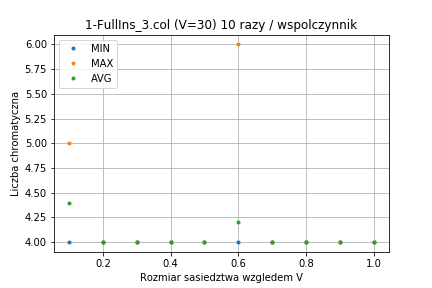
\includegraphics[width = 2.8in]{1-FullIns3}} &
\subfloat{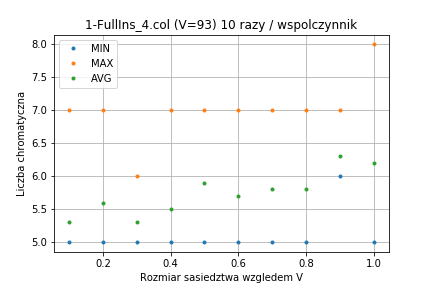
\includegraphics[width = 2.8in]{1-FullIns4}} \\
\subfloat{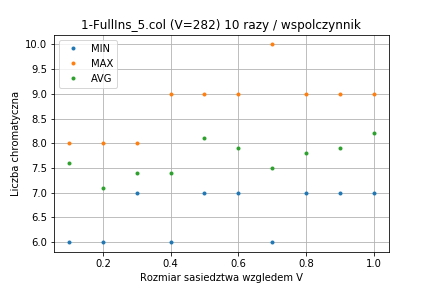
\includegraphics[width = 2.8in]{1-FullIns5}} &
\subfloat{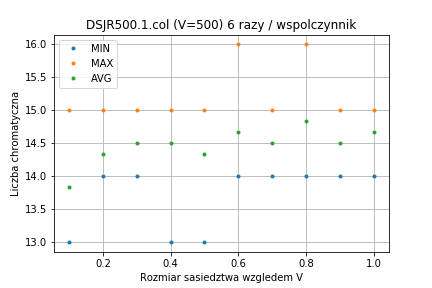
\includegraphics[width = 2.8in]{DSJR500}} \\
\subfloat{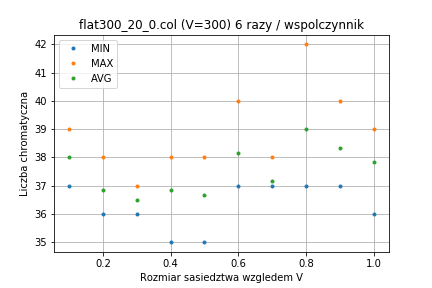
\includegraphics[width = 2.8in]{flat300}} &
\subfloat{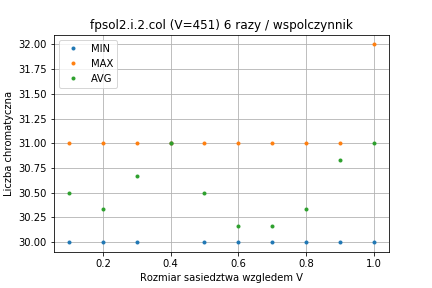
\includegraphics[width = 2.8in]{fpsol2}} \\
\subfloat{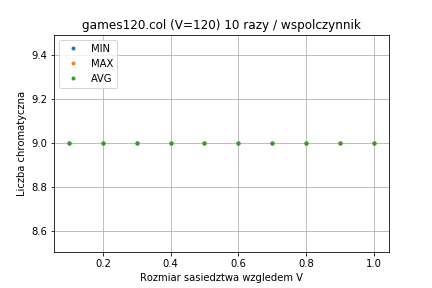
\includegraphics[width = 2.8in]{games120}} &
\subfloat{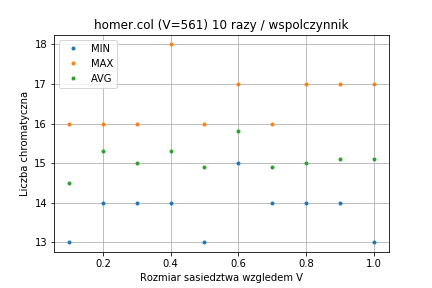
\includegraphics[width = 2.8in]{homer}} \\
\end{tabular}
\label{fig:n1}
\caption{Badanie rozmiaru sąsiedztwa}
\end{figure}

\begin{figure}  [H]
\begin{tabular}{cc}

\subfloat{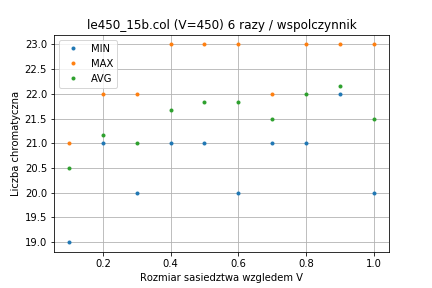
\includegraphics[width = 2.8in]{le450}} &
\subfloat{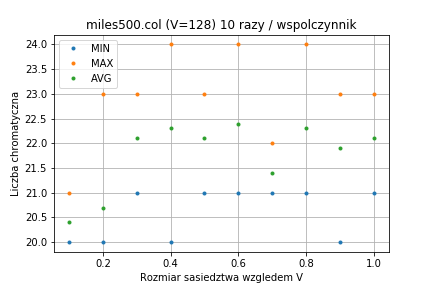
\includegraphics[width = 2.8in]{miles500}} \\
\subfloat{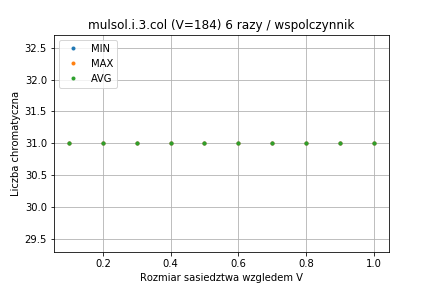
\includegraphics[width = 2.8in]{mulsol}} &
\subfloat{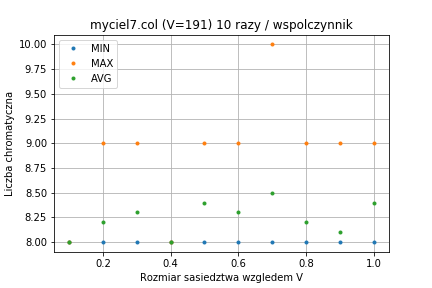
\includegraphics[width = 2.8in]{myciel7}} \\
\subfloat{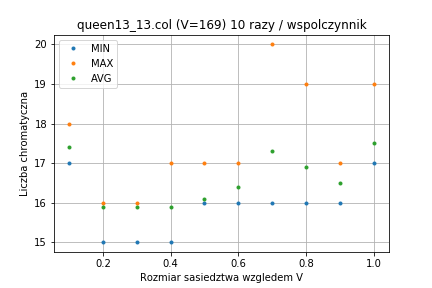
\includegraphics[width = 2.8in]{queen13}} &
\subfloat{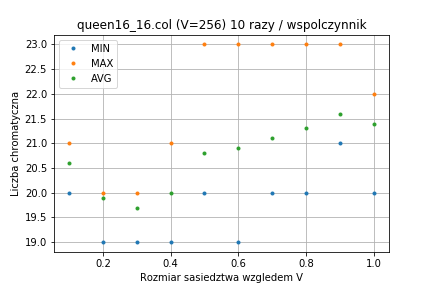
\includegraphics[width = 2.8in]{queen16}} \\
\subfloat{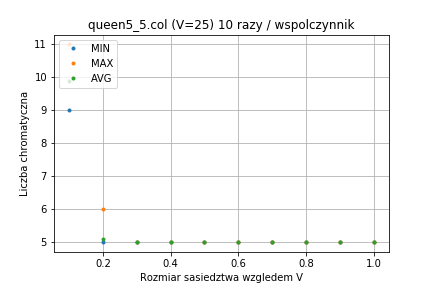
\includegraphics[width = 2.8in]{queen5}} &
\subfloat{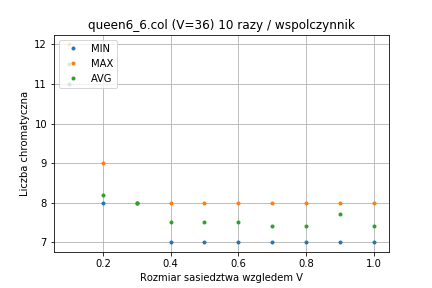
\includegraphics[width = 2.8in]{queen6}} \\

\end{tabular}
\label{n2}
\caption{Badanie rozmiaru sąsiedztwa c.d.}
\end{figure}

\textit{TODO: Wnioski z badania rozmiaru sąsiedztwa}

\subsubsection{Badanie rozmiaru listy tabu}
\textit{TODO: wykres z badania rozmiaru listy tabu}
\subsubsection{Początkowa liczba kolorów}
\textit{TODO: Tutaj te spostrzeżenia o początkowej liczbie kolorów, można coś napisać o tej eksploracji i eksploatacji}

\subsection{Wyniki poszukiwań liczby chromatycznej}
\textit{TODO: opisać czym są poszczególne rodziny grafów}


\begin{figure} [H]
\begin{tabular}{|c|c|c|c|c|c|}%
	\hline
    \bfseries Graph & V & E & Faktyczne $\chi$ & Najlepsze $\chi$ z artykułu & \bfseries Tabu $\chi$
    \csvreader[head to column names]{resources/queensResults.csv}{}% use head of csv as column names
    {\\\hline \Graph & \V & \E & \Chrom & \ArticleBest & \bfseries\TabuBest}% specify your coloumns here
    \\ \hline
\end{tabular}
\caption{Pomiary dla grafów typu queens}
\end{figure}

\begin{figure} [H]
\begin{tabular}{|c|c|c|c|c|c|}%
	\hline
    \bfseries Graph & V & E & Faktyczne $\chi$ & Najlepsze $\chi$ z artykułu & \bfseries Tabu $\chi$
    \csvreader[head to column names]{resources/leightonResults.csv}{}% use head of csv as column names
    {\\\hline \graph & \v & \e & \chrom & \art & \bfseries\tabu}% specify your coloumns here
    \\ \hline
\end{tabular}
\caption{Pomiary dla grafów Leightona}
\end{figure}

\begin{figure} [H]
\begin{tabular}{|c|c|c|c|c|c|}%
	\hline
    \bfseries Graph & V & E & Faktyczne $\chi$ & Najlepsze $\chi$ z artykułu & \bfseries Tabu $\chi$
    \csvreader[head to column names]{resources/mycielResults.csv}{}% use head of csv as column names
    {\\\hline \graph & \v & \e & \chrom & \art & \bfseries\tabu}% specify your coloumns here
    \\ \hline
\end{tabular}
\caption{Pomiary dla grafów Mycielskiego}
\end{figure}

\begin{figure} [H]
\begin{tabular}{|c|c|c|c|c|c|}%
	\hline
    \bfseries Graph & V & E & Faktyczne $\chi$ & Najlepsze $\chi$ z artykułu & \bfseries Tabu $\chi$
    \csvreader[head to column names]{resources/racResults.csv}{}% use head of csv as column names
    {\\\hline \graph & \v & \e & \chrom & \art & \bfseries\tabu}% specify your coloumns here
    \\ \hline
\end{tabular}
\caption{Pomiary dla grafów rac}
\end{figure}  
    
\begin{figure} [H]
\begin{tabular}{|c|c|c|c|c|c|}%
	\hline
    \bfseries Graph & V & E & Faktyczne $\chi$ & Najlepsze $\chi$ z artykułu & \bfseries Tabu $\chi$
    \csvreader[head to column names]{resources/randomResults.csv}{}% use head of csv as column names
    {\\\hline \graph & \v & \e & \chrom & \art & \bfseries\tabu}% specify your coloumns here
    \\ \hline
\end{tabular}
\caption{Pomiary dla grafów losowych}
\end{figure}  

\begin{figure} [H]
\begin{tabular}{|c|c|c|c|c|c|}%
	\hline
    \bfseries Graph & V & E & Faktyczne $\chi$ & Najlepsze $\chi$ z artykułu & \bfseries Tabu $\chi$
    \csvreader[head to column names]{resources/carResults.csv}{}% use head of csv as column names
    {\\\hline \graph & \v & \e & \chrom & \art & \bfseries\tabu}% specify your coloumns here
    \\ \hline
\end{tabular}
\caption{Pomiary dla grafów car}
\end{figure}  



\bibliography{sources}
\nocite{*}
\bibliographystyle{plain}

\end{document}